%
% Main document
% ===========================================================================
% This is part of the document "Project documentation template".
% Authors: brd3, kaa1
%

%---------------------------------------------------------------------------
\documentclass[
	a4paper,					% paper format
	12pt,							% fontsize
%	twoside,					% double-sided
	openright,				% begin new chapter on right side
	notitlepage,			% use no standard title page
	parskip=half,			% set paragraph skip to half of a line
]{scrreprt}					% KOMA-script report
%---------------------------------------------------------------------------

\raggedbottom
\KOMAoptions{cleardoublepage=plain}			% Add header and footer on blank pages


% Load Standard Packages:
%---------------------------------------------------------------------------
\usepackage[standard-baselineskips]{cmbright}

\usepackage[ngerman]{babel}										% german hyphenation
\usepackage{afterpage}
%\usepackage[latin1]{inputenc}  							% Unix/Linux - load extended character set (ISO 8859-1)
\usepackage[ansinew]{inputenc}  							% Windows - load extended character set (ISO 8859-1)
\usepackage[T1]{fontenc}											% hyphenation of words with �,� and �
\usepackage{textcomp}													% additional symbols
\usepackage{longtable}
\usepackage{ae}																% better resolution of Type1-Fonts 
\usepackage{nameref}
\usepackage{floatrow}
\usepackage{wrapfig}
\usepackage{fancyhdr}													% simple manipulation of header and footer 
\usepackage{etoolbox}													% color manipulation of header and footer
\usepackage{graphicx}                      		% integration of images
\usepackage{float}														% floating objects
\usepackage{caption}													% for captions of figures and tables
\usepackage{booktabs}													% package for nicer tables
\usepackage{tocvsec2}													% provides means of controlling the sectional numbering
\usepackage{array}
\usepackage{rotating}
%\usepackage{svg}
%---------------------------------------------------------------------------

% Load Math Packages
%---------------------------------------------------------------------------
\usepackage{amsmath}                    	   	% various features to facilitate writing math formulas
\usepackage{amsthm}                       	 	% enhanced version of latex's newtheorem
\usepackage{amsfonts}                      		% set of miscellaneous TeX fonts that augment the standard CM
\usepackage{amssymb}													% mathematical special characters
\usepackage{exscale}													% mathematical size corresponds to textsize
%---------------------------------------------------------------------------

% Package to facilitate placement of boxes at absolute positions
%---------------------------------------------------------------------------
\usepackage[absolute]{textpos}
\setlength{\TPHorizModule}{1mm}
\setlength{\TPVertModule}{1mm}
%---------------------------------------------------------------------------					
			
% Definition of Colors
%---------------------------------------------------------------------------
\RequirePackage{color}                          % Color (not xcolor!)
\definecolor{linkblue}{rgb}{0,0,0.8}            % Standard
\definecolor{darkblue}{rgb}{0,0.08,0.45}        % Dark blue
\definecolor{bfhgrey}{rgb}{0.41,0.49,0.57}      % BFH grey
%\definecolor{linkcolor}{rgb}{0,0,0.8}     			% Blue for the web- and cd-version!
\definecolor{linkcolor}{rgb}{0,0,0}        			% Black for the print-version!
%---------------------------------------------------------------------------

% Hyperref Package (Create links in a pdf)
%---------------------------------------------------------------------------
\usepackage[
	pdftex,ngerman,bookmarks,plainpages=false,pdfpagelabels,
	backref = {false},										% No index backreference
	colorlinks = {true},                  % Color links in a PDF
	hypertexnames = {true},               % no failures "same page(i)"
	bookmarksopen = {true},               % opens the bar on the left side
	bookmarksopenlevel = {0},             % depth of opened bookmarks
	pdftitle = {Template f�r Bachelor Thesis},	   	% PDF-property
	pdfauthor = {brd3},        					  % PDF-property
	pdfsubject = {LaTeX Template},        % PDF-property
	linkcolor = {linkcolor},              % Color of Links
	citecolor = {linkcolor},              % Color of Cite-Links
	urlcolor = {linkcolor},               % Color of URLs
]{hyperref}
%---------------------------------------------------------------------------
% Set up page dimension
%---------------------------------------------------------------------------
\usepackage{geometry}
\geometry{
	a4paper,
	left=28mm,
	right=15mm,
	top=30mm,
	headheight=20mm,
	headsep=10mm,
	textheight=242mm,
	footskip=15mm
}
%---------------------------------------------------------------------------

% Makeindex Package
%---------------------------------------------------------------------------
\usepackage{makeidx}                         		% To produce index
\makeindex                                    	% Index-Initialisation
%---------------------------------------------------------------------------

% Glossary Package
%---------------------------------------------------------------------------
% the glossaries package uses makeindex
% if you use TeXnicCenter do the following steps:
%  - Goto "Ausgabeprofile definieren" (ctrl + F7)
%  - Select the profile "LaTeX => PDF"
%  - Add in register "Nachbearbeitung" a new "Postprozessoren" point named Glossar
%  - Select makeindex.exe in the field "Anwendung" ( ..\MiKTeX x.x\miktex\bin\makeindex.exe )
%  - Add this [ -s "%tm.ist" -t "%tm.glg" -o "%tm.gls" "%tm.glo" ] in the field "Argumente"
%
% for futher informations go to http://ewus.de/tipp-1029.html
%---------------------------------------------------------------------------
\usepackage[nonumberlist]{glossaries}
\makeglossaries
\usepackage{xparse}
\DeclareDocumentCommand{\newdualentry}{ O{} O{} m m m m } {
	\newglossaryentry{gls-#3}{name={#5},text={#5\glsadd{#3}},
		description={#6},#1
	}
	\newacronym[type=\acronymtype, see={[Glossary:]{gls-#3}},#2]{#3}{#4}{#5\glsadd{gls-#3}}
}


% GLOSSARY
\newglossaryentry{imvr}{name={IMVR},description={Kurz f�r ``Images \& Music in VR''. Die Applikation, die im Rahmen dieses Projekts mit Unity 5 entwickelt wird}}
\newglossaryentry{unity}{name={Unity},description={Unity ist eine Spielengine, die das einfache Entwickeln von 3D-Applikation f�r diverse Endger�te erlaubt}}
\newglossaryentry{rift}{name={Oculus Rift},description={Ein \gls{hmd} von Oculus VR}}
\newglossaryentry{leap}{name={Leap Motion},description={Ein auf Infrarotkameras basierter Handerkennungs-Sensor}}


% ACRONYMS
\newacronym[type=\acronymtype]{hmd}{HMD}{Head-Mounted Display}
\newacronym{vr}{VR}{Virtual Reality}
%\newglossaryentry{ipd}{name={IPD},description={Beschreibt den Augenabstand.}}
\newdualentry{ipd}{IPD}{Inter-Pupillary Distance}{Beschreibt den Augenabstand und stellt ein wichtiges Mass f�r die stereoskopische Darstellung von Bildern dar}
%---------------------------------------------------------------------------

% Intro:
%---------------------------------------------------------------------------
\begin{document}                              	% Start Document
\settocdepth{section}														% Set depth of toc
\pagenumbering{roman}														
%---------------------------------------------------------------------------
\providecommand{\titel}{Bringing Your Hands Into Virtual Reality}		%  Hier den Titel des Berichts/Thesis eingeben					% Titel der Arbeit aus Datei titel.tex lesen
\providecommand{\versionnumber}{1.0}			%  Hier die aktuelle Versionsnummer eingeben
\providecommand{\versiondate}{11.06.2015}		%  Hier das Datum der aktuellen Version eingeben				% Versionsnummer und -datum aus Datei version.tex lesen

% Set up header and footer
%---------------------------------------------------------------------------
\makeatletter
\patchcmd{\@fancyhead}{\rlap}{\color{bfhgrey}\rlap}{}{}		% new color of header
\patchcmd{\@fancyfoot}{\rlap}{\color{bfhgrey}\rlap}{}{}		% new color of footer
\makeatother

\fancyhf{}																		% clean all fields
\fancypagestyle{plain}{												% new definition of plain style	
	\fancyfoot[OR,EL]{\footnotesize \thepage} 	% footer right part --> page number
	\fancyfoot[OL,ER]{\footnotesize \titel, Version \versionnumber, \versiondate}	% footer even page left part 
}

\renewcommand{\chaptermark}[1]{\markboth{\thechapter.  #1}{}}
\renewcommand{\headrulewidth}{0pt}				% no header stripline
\renewcommand{\footrulewidth}{0pt} 				% no bottom stripline

\pagestyle{plain}

%---------------------------------------------------------------------------


% Title Page and Abstract
%---------------------------------------------------------------------------
\newgeometry{twoside}
%%
% Project documentation template
% ===========================================================================
% This is part of the document "Project documentation template".
% Authors: brd3, kaa1
%

\begin{titlepage}


% BFH-Logo absolute placed at (28,12) on A4 
% Actually not a realy satisfactory solution but working.
%---------------------------------------------------------------------------
\setlength{\unitlength}{1mm}
\begin{textblock}{20}[0,0](28,12)
	
\includegraphics[scale=1.0]{bilder/BFH_Logo_B.png}
\end{textblock}
\color{black}

% Institution / Titel / Untertitel / Autoren / Experten:
%---------------------------------------------------------------------------
\begin{flushleft}

\vspace*{21mm}

\fontsize{26pt}{40pt}\selectfont 
\titel 				\\							% Titel aus der Datei vorspann/titel.tex lesen
\vspace{2mm}

\fontsize{16pt}{24pt}\selectfont\vspace{0.3em}
Hier steht ein Untertitel 			\\							% Untertitel eingeben
\vspace{5mm}

\fontsize{10pt}{12pt}\selectfont
\textbf{Art der Arbeit (Semesterarbeit / Bachelorthesis / etc.)} \\									% eingeben
\vspace{7mm}

% Abstract (eingeben):
%---------------------------------------------------------------------------
\begin{textblock}{150}(28,100)
\fontsize{10pt}{12pt}\selectfont
[Kurztext (Abstract) einf�gen, falls gew�nscht] \\ 
Dieses Dokument dient als Vorlage f�r die Erstellung von Berichten nach den Richtlinien der BFH. Die Vorlage ist in \LaTeX{} erstellt und unterst�tzt das automatische Erstellen von diversen Verzeichnissen, Literaturangaben, Indexierung und Glossaren. Dieser kleine Text ist eine Zusammenfassung �ber das vorliegenden Dokument mit einer L�nge von 4 bis max. 8 Zeilen. \\
Das Titelbild kann in den Zeilen 157/158 der Datei template.tex ein- oder ausgeschaltet werden.
\end{textblock}

\begin{textblock}{150}(28,225)
\fontsize{10pt}{17pt}\selectfont
\begin{tabbing}
xxxxxxxxxxxxxxx\=xxxxxxxxxxxxxxxxxxxxxxxxxxxxxxxxxxxxxxxxxxxxxxx \kill
Studiengang:	\> [z.B. Elektro- und Kommunikationstechnik]	\\			% Namen eingeben
Autoren:		\> [Test Peter, M�ster R�s�]		\\					% Namen eingeben
Betreuer:	\> [Dr.~Xxxx Xxxx, Dr.~Yyyy Yyyy]		\\					% Namen eingeben
Auftraggeber:	\> [Wwwww AG]						\\					% Namen eingeben
Experten:		\> [Dr.~Zzzz Zzzz]				\\					% Namen eingeben
Datum:			\> \versiondate					\\		% aus Datei vorspann/version.tex lesen
\end{tabbing}

\end{textblock}
\end{flushleft}

\begin{textblock}{150}(28,280)
\noindent 
\color{bfhgrey}\fontsize{9pt}{10pt}\selectfont
Berner Fachhochschule | Haute �cole sp�cialis�e bernoise | Bern University of Applied Sciences
\color{black}\selectfont
\end{textblock}


\end{titlepage}

%
% ===========================================================================
% EOF
%
		% activate for Titelseite ohne Bild
%
% Project documentation template
% ===========================================================================
% This is part of the document "Project documentation template".
% Authors: brd3, kaa1
%

\begin{titlepage}


% BFH-Logo absolute placed at (28,12) on A4 and picture (16:9 or 15cm x 8.5cm)
% Actually not a realy satisfactory solution but working.
%---------------------------------------------------------------------------
\setlength{\unitlength}{1mm}
\begin{textblock}{20}[0,0](28,12)
	
\includegraphics[scale=1.0]{bilder/BFH_Logo_B.png}
\end{textblock}

\begin{textblock}{154}(28,48)
	\begin{picture}(150,2)
		\put(0,0){\color{bfhgrey}\rule{150mm}{2mm}}
	\end{picture}
\end{textblock}

\begin{textblock}{154}[0,0](28,55)
	\centering
	
\includegraphics[width=0.7\linewidth]{bilder/logo}			% Titelbild definieren
\end{textblock}

\begin{textblock}{154}(28,155)
	\begin{picture}(150,2)
		\put(0,0){\color{bfhgrey}\rule{150mm}{2mm}}
	\end{picture}
\end{textblock}
\color{black}

% Institution / Titel / Untertitel / Autoren / Experten:
%---------------------------------------------------------------------------
\begin{flushleft}

\vspace*{125mm}

\fontsize{26pt}{28pt}\selectfont 
\titel 				\\							% Titel aus der Datei vorspann/titel.tex lesen
\vspace{2mm}

\fontsize{16pt}{20pt}\selectfont\vspace{0.3em}
Schlussbericht 			\\							% Untertitel eingeben
\vspace{5mm}

\fontsize{10pt}{12pt}\selectfont
%\textbf{Art der Arbeit (Semesterarbeit / Bachelorthesis / etc.)} \\									% eingeben
\vspace{3mm}

% Abstract (eingeben):
%---------------------------------------------------------------------------
%\begin{textblock}{150}(28,190)
%\fontsize{10pt}{12pt}\selectfont
%[Kurztext (Abstract) einf�gen, falls gew�nscht] \\ 
%Dieses Dokument dient als Vorlage f�r die Erstellung von Berichten nach den Richtlinien der BFH. Die Vorlage ist in \LaTeX{} erstellt und unterst�tzt das automatische Erstellen von diversen Verzeichnissen, Literaturangaben, Indexierung und Glossaren. Dieser kleine Text ist eine Zusammenfassung �ber das vorliegenden Dokument mit einer L�nge von 4 bis max. 8 Zeilen. \\
%Das Titelbild kann in den Zeilen 157/158 der Datei template.tex ein- oder ausgeschaltet werden.
%\end{textblock}

\begin{textblock}{150}(28,225)
\fontsize{10pt}{17pt}\selectfont
\begin{tabbing}
xxxxxxxxxxxxxxx\=xxxxxxxxxxxxxxxxxxxxxxxxxxxxxxxxxxxxxxxxxxxxxxx \kill
Studiengang:	\> Informatik	\\			% Namen eingeben
Autoren:		\> Simon Meer		\\					% Namen eingeben
Betreuer:	\> Prof. Urs K�nzler		\\					% Namen eingeben
%Auftraggeber:	\> [Wwwww AG]						\\					% Namen eingeben
Experten:		\> Yves Petitpierre				\\					% Namen eingeben
Datum:			\> \versiondate					\\		% aus Datei vorspann/version.tex lesen
\end{tabbing}

\end{textblock}
\end{flushleft}

\begin{textblock}{150}(28,280)
\noindent 
\color{bfhgrey}\fontsize{9pt}{10pt}\selectfont
Berner Fachhochschule | Haute �cole sp�cialis�e bernoise | Bern University of Applied Sciences
\color{black}\selectfont
\end{textblock}


\end{titlepage}

%
% ===========================================================================
% EOF
%
			% activate for Titelseite mit Bild
% Versionenkontrolle :
% -----------------------------------------------
%\pagebreak
\begin{textblock}{180}(15,150)
\color{black}
\begin{huge}
Versionen
\end{huge}
\vspace{10mm}

\fontsize{10pt}{18pt}\selectfont
\begin{tabbing}
xxxxxxxxxxx\=xxxxxxxxxxxxxxx\=xxxxxxxxxxxxxx\=xxxxxxxxxxxxxxxxxxxxxxxxxxxxxxxxxxxxxxxxxxxxxxx \kill
Version	\> Datum	\> Status		\> Bemerkungen		\\
0.9	\> 14.04.2015	\> Entwurf		\> Outline erstellt	\\
\end{tabbing}

\end{textblock}
%\pagebreak
\cleardoubleemptypage
\restoregeometry
\setcounter{page}{1}
%\cleardoublepage
%\phantomsection 
%\addcontentsline{toc}{chapter}{Management Summary}
%\chapter*{Management Summary}
\label{chap:managementSummary}

Lorem ipsum dolor sit amet, consectetur adipiscing elit. Phasellus scelerisque, leo sed iaculis ornare, mi leo semper urna, ac elementum libero est at risus. Donec eget aliquam urna. Lorem ipsum dolor sit amet, consectetur adipiscing elit. Nunc fermentum nunc sollicitudin leo porttitor volutpat. Duis ac enim lectus, quis malesuada lectus. Aenean vestibulum suscipit justo, in suscipit augue venenatis a. Donec interdum nibh ligula. Aliquam vitae dui a odio cursus interdum quis vitae mi. Phasellus ornare tortor fringilla velit accumsan quis tincidunt magna eleifend. Praesent nisl nibh, cursus in mattis ac, ultrices ac nulla. Nulla ante urna, aliquet eu tempus ut, feugiat id nisl. Nunc sit amet mauris vitae turpis scelerisque mattis et sed metus. Aliquam interdum congue odio, sed semper elit ullamcorper vitae. Morbi orci elit, feugiat vel hendrerit nec, sollicitudin non massa. Quisque lacus metus, vulputate id ullamcorper id, consequat eget orci \nocite{kopka:band1} \nocite{Marti06}. 

\cleardoubleemptypage
%---------------------------------------------------------------------------

% Table of contents
%---------------------------------------------------------------------------
\tableofcontents
\cleardoublepage
%---------------------------------------------------------------------------

% Main part:
%---------------------------------------------------------------------------
\pagenumbering{arabic}

\chapter{Einleitung}
\label{chap:einleitung}

Der Markt der stereoskopischen Brillen befindet sich in einem starken Wachstum. Oculus Rift, SteamVR, Project Morpheus, Nvidia VR - die Liste der teilnehmenden Partien w�chst und w�chst, doch neue Ausgabeger�te ben�tigen auch neue Eingabeger�te. Die Leap Motion kann als ein solches gez�hlt werden und bietet eine freie Handerkennung ohne irgendwelche Handschuhe tragen zu m�ssen.

In diesem Projekt geht es darum, die neuartige Eingabem�glichkeiten der Leap Motion in Verbindung mit der Oculus Rift einzusetzen und damit eine interaktive \gls{vr}-Applikation zu schreiben. Im Rahmen eines vorhergehenden Projekts wurde die Materie bereits bearbeitet und die M�glichkeiten erforscht. Es geht nun also haupts�chlich um die erfolgreiche Anwendung der erarbeiteten Informationen.
\chapter{Vision ``IMVR''}

Die Vision soll dazu dienen, einen �berblick �ber die Applikation zu geben, die im Rahmen der Bachelorarbeit erstellt wird.

\section{Problemstellung}

Es soll eine Applikation namens ``\gls{imvr}'' entwickelt werden, welche Gebrauch von der Oculus Rift macht, um die Bilder- und Musiksammlung des Anwenders ansprechend darzustellen, z.B. in Form eines 3D-Karussels. Die zus�tzliche "Tiefe", die durch den Einsatz eines stereoskopischen \gls{hmd} entsteht, soll dem Anwender helfen, sich in seiner Medienbibliothek schneller zurechtzufinden.

Zus�tzlich dazu soll die Leap Motion dazu verwendet werden, um vollst�ndige Handfreiheit zu gew�hren: Der Anwender soll komplett ohne Maus und Tastatur imstande sein, sich durch seine Bilder zu navigieren.

Kurz zusammengefasst muss die Applikation:

\begin{itemize}
	\item Die Bild- und Musikbibliothek des Benutzers in stereoskopischem 3D darstellen.
	\item Diese freih�ndig durchsuchbar machen mit Sortier- und evtl. Gruppierfunktion.
	\item Die Bilder betrachtbar und die Musik abspielbar machen.
	\item Metainformationen darstellen (z.B. in Form von Diagrammen).
\end{itemize}

Zus�tzlich zur Applikation selbst soll noch ein zus�tzliches Tool entwickelt werden, welches im Voraus die Dateien auf dem Host-System indexiert und f�r die visuelle Applikation bereitstellt.

\section{Technologien}

Das Projekt verwendet spezielle Hardware und Software. Es folgt eine kurze Erkl�rung zu diesen Technologien.

\subsection{Oculus Rift}

Die Oculus Rift ist ein stereoskopisches \gls{hmd}, welches durch Oculus VR entwickelt wird. Die aktuelle Version ist das Developer Kit 2 (DK2). Ein Termin f�r die finale Version steht noch nicht fest.

Hardwarem�ssig besteht die Rift aus einem Headset f�r das Bild und einer Kamera f�r das Head-Tracking. Das Headset wird per USB und HDMI an den Computer angeschlossen und �ber ein Stromkabel mit Strom versorgt. Die Kamera wird auf dem Computerbildschirm platziert, und per USB an den Computer und per Sync-Kabel an die Rift angeschlossen.

\begin{figure}[h]
\centering
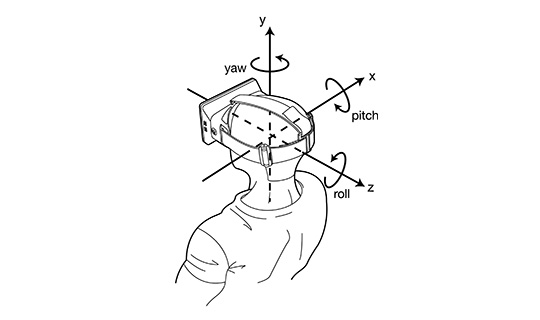
\includegraphics[width=0.7\linewidth]{bilder/rift1}
\caption{Illustration, welche die Anwendung und das Koordinatensystem der Oculus Rift verdeutlicht.}
\floatfoot{Quelle: \url{https://www.oculus.com/blog/building-a-sensor-for-low-latency-vr/}}
\label{fig:rift1}
\end{figure}

Seit DK2 ist das Headset mit 40 Infrarot-LEDs best�ckt, welche mit einer bestimmten Frequenz aufleuchten und von der Kamera f�r das Head-Tracking benutzt werden.
 
Auf der Software-Seite wird ein Treiber auf dem Computer installiert, der nach einer Registration als Entwickler auf der offiziellen Seite erh�ltlich ist . Die Software erlaubt die Erstellung von Benutzerprofilen, um die \gls{ipd} korrekt einzustellen. Es ist ausserdem m�glich, zwischen zwei Betriebsmodi auszuw�hlen: dem traditionellen Modus, wo die Rift als zweiter Bildschirm angesprochen wird, und dem neuen ``Direct Mode'', wo die Rift direkt angesprochen wird.

\subsection{Leap Motion}

Die \gls{leap} besteht aus einem rechteckigen Ger�t mit zwei Infrarotsensoren, welche deren Daten per USB auf den angeschlossenen Computer �bertr�gt. Nach der Installation der Leap Motion Runtime l�uft auf dem Computer ein Service, der diese Daten empf�ngt, verarbeitet und per API mit einer variablen Framerate verschiedenen Applikationen zur Verf�gung stellt.

Die Daten, welche diese API liefert, sind in sogenannte ``Frames'' gruppiert. Ein Frame ist sozusagen eine Momentaufnahme der Realit�t, welche sich aus erkannten H�nden zusammensetzt. Durchschnittlich werden pro Sekunde etwa um die 100 dieser Frames berechnet.

\begin{figure}[H]
	\centering
	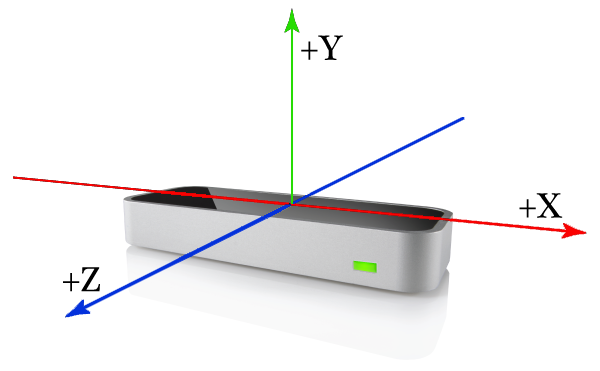
\includegraphics[width=0.7\linewidth]{bilder/leap1}
	\caption{Verdeutlichung des Koordinatensystems.}
	\floatfoot{Quelle: \url{https://developer.leapmotion.com/documentation/csharp/devguide/Leap_Coordinate_Mapping.html}}
	\label{fig:leap1}
\end{figure}

Durch diese Frames kann man auf die Daten der H�nde zugreifen. Jede Hand erh�lt eine ID, womit man gleiche H�nde Frame-�bergreifend identifizieren kann, sowie die dazugeh�renden Koordinaten und Drehungen. Auf Abbildung \ref{fig:leap1} wird ersichtlich, dass sich die Koordinaten in einem rechtsh�ndigen Koordinatensystem befinden, wobei die Y-Achse nach oben zeigt und die Masse in Millimeter angegeben sind. Die Koordinaten der Finger sind innerhalb von Finger-Instanzen gruppiert, welche wiederum ihre Gelenke als Instanzen einer Joint-Klasse zur Verf�gung stellen.

\begin{figure}[H]
	\centering
	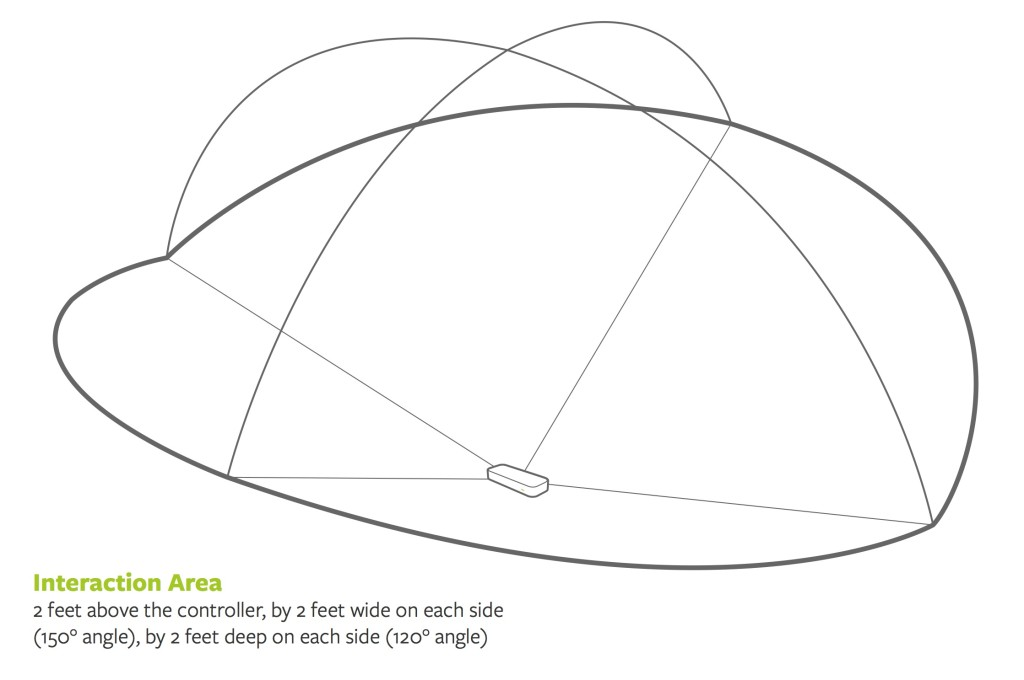
\includegraphics[width=0.7\linewidth]{bilder/leap2}
	\caption{Das Sichtfeld der Leap Motion.}
	\floatfoot{Quelle: \url{https://community.leapmotion.com/t/accurately-measuring-distances/842/3 }}
	\label{fig:leap2}
\end{figure}

Die Leap Motion hat ungef�hr eine Reichweite von einem Meter, wobei das Interaktionsfeld einer Form, wie in Abbildung \ref{fig:leap2} ersichtlich ist, entspricht. Das Sichtfeld liegt bei 150� in vertikaler und 120� in horizontaler Richtung.


\subsection{Unity 5}

\gls{unity} ist eine Entwicklungsumgebung und eine Spiel-Engine, die momentan aufgrund ihrer Bedienungsfreundlichkeit und einer frei erh�ltlichen Version sehr beliebt in der Szene der Indie-Developer ist. Gleichzeitig dient sie auch als gutes Prototyping-Tool, um schnell Ideen umzusetzen.

Am 3. M�rz 2015 machte Unity einen Versionssprung und ist nun unter dem Namen ``Unity 5'' erh�ltlich. Neben anderen Neuerungen sind jetzt alle Funktionen, f�r die fr�her eine kostenpflichtige Lizenz erworben werden musste, auch in der freien Version erh�ltlich, was f�r dieses Projekt einen gr�sseren Spielraum bedeutet.

In diesem Projekt wurde Unity wegen der angenehmen Lernkurve und der guten Integrierung mit der Oculus Rift und der Leap Motion f�r den Einsatz gew�hlt. Wie bereits erw�hnt wurde, ist es leicht, schnell zu Ergebnissen zu kommen, und die Entwicklungsumgebung unterst�tzt die zwei Programmiersprachen, die der Verfasser dieses Dokuments am besten beherrscht.

\section{Anwendung}

Innerhalb von \gls{imvr} wird die Leap Motion mit einer Halterung an der Oculus Rift befestigt, welche auf der offiziellen Website von Leap Motion f�r rund \$15\footnote{Siehe \url{https://www.leapmotion.com/product/vr}} erh�ltlich ist. Wie in Abbildung \ref{fig:uebersicht} ersichtlich ist, sind beide Ger�te unter Anderem per USB am PC befestigt und senden dar�ber ihre Daten an die entsprechenden Services. Diese leiten wiederum die ausgewerteten Daten durch �ffentliche APIs an Unity bzw. IMVR weiter.

\afterpage {
\begin{figure}[t!]
	\centering
	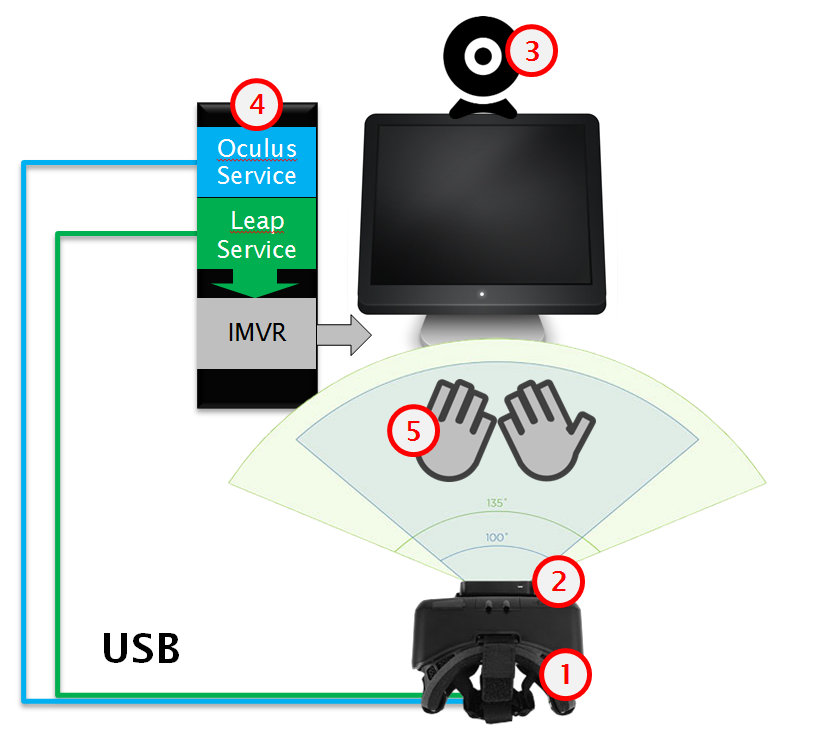
\includegraphics[width=0.8\linewidth]{bilder/systemuebersicht}
	\caption{Eine �bersicht der Technologien und wie sie verbunden sind.}
	\label{fig:uebersicht}
\end{figure}

\begin{table}[H]
	\centering
	\begin{tabular}{p{0.1\linewidth} p{0.3\linewidth} p{0.5\linewidth}}
		\textbf{Nr.} & \textbf{Komponente} & \textbf{Beschreibung} \\ \midrule
		1. & Oculus Rift DK2 & \gls{hmd} f�r den grafischen Output. \\
		2. & Leap Motion & Ger�t, welches H�nde erkennt und ihre Koordinaten an den Computer sendet. \\
		3. & Oculus Rift Kamera & Kamera, welche seit dem DK2 f�r das �rtliche Tracking zust�ndig ist. \\
		4. & Computer & Host-System f�r IMVR. \\
		5. & Benutzer & Benutzer, der die Oculus Rift tr�gt und mit seinen H�nden das Programm steuert. \\
	\end{tabular}
\end{table}
}

\clearpage
\chapter{Spezifikationen}

In diesem Kapitel sollen die Anforderungen, die in der Vision grob geschildert wurden, konkretisiert und aufgelistet werden.

\section{Funktionale Anforderungen}

In der folgenden Tabelle sind alle Anforderungen aufgelistet mit einer Priorit�t von 1 bis 5, wobei eine tiefere Zahl f�r eine h�here Priorit�t steht. Grunds�tzlich kann gesagt werden, dass alle Anforderungen, die mit einer 1 deklariert werden, implementiert werden m�ssen und alle Anforderungen, die mit einer 5 deklariert werden, nur Ideen sind, welche mit hoher Wahrscheinlichkeit nicht implementiert werden k�nnen.

%\begin{table}[H]
	\begin{longtable}{p{0.06\textwidth} p{0.7\textwidth} p{0.13\textwidth}} \toprule %{p{0.13\textwidth} p{0.75\textwidth}} \toprule
		\textbf{Nr.} & \textbf{Beschreibung} & \textbf{Priorit�t} \\ \midrule
		\endhead
		\multicolumn{3}{l}{\textbf{1. Elementares}} \\ \midrule
		1.1 & Die Applikation nutzt die Oculus Rift im direkten Modus f�r die Ausgabe. & 1 \\
		1.2 & Die Applikation ist vollst�ndig mit den H�nden bedienbar. & 1 \\
		1.3 & Die Applikation erlaubt den Zugriff auf alle gefundenen, validen Dateien. & 1 \\
		1.4 & Bilder k�nnen angeschaut werden, Musik kann angeh�rt werden. & 1 \\
		1.5 & Die Hintergrundmusik kann von der Musikbibliothek ausgew�hlt werden. & 2 \\
		1.6 & Die Applikation kann jederzeit beendet werden. & 1 \\
		1.7 & H�nde werden abstrakt dargestellt. & 2 \\
		1.8 & Die Applikation erreicht eine stetige Framerate von mindestens 60fps auf dem Referenzsystem\footnote{Intel(R) Xeon CPU E5-1650 v3 @ 2.50Ghz mit 32GB RAM und einer NVIDIA GeForce GTX 980 Grafikkarte.}. & 1 \\
		\multicolumn{3}{l}{\textbf{2. �bersicht (Bilder)}} \\ \nopagebreak \midrule
		2.1 & Elemente k�nnen in einem 3D-Karussell dargestellt werden. & 1 \\
		2.2 & Elemente k�nnen selektiert werden. & 2 \\
		2.3 & Elemente k�nnen getaggt werden. & 3 \\
		2.4 & Es kann auf ein bestimmtes Element fokussiert werden (siehe Detailansicht). & 1 \\
		2.5 & Es ist eine Mehrfachselektierung m�glich. & 3 \\
		2.6 & Elemente k�nnen in anderen Anordnungen dargestellt werden (Tunnel, Fluss, Fl�che, W�rfel, etc.) & 3 \\
		2.7 & Bilder k�nnen nach Farbton, S�ttigung und Helligkeit sortiert werden. & 1 \\
		2.8 & Bilder k�nnen alphabetisch und chronologisch sortiert werden. & 2 \\
		2.9 & Bilder k�nnen nach Dateiordner gruppiert werden. & 3 \\
		2.10& Bilder k�nnen nach Kennwerten (Varianz, Entropie) sortiert werden & 3 \\
		\multicolumn{3}{l}{\textbf{3. Detailansicht (Bilder)}} \\ \nopagebreak \midrule
		3.1 & Bild kann vergr�ssert und verkleinert werden. & 1 \\
		3.2 & Bild kann gel�scht werden & 2 \\
		3.3 & Ein (3D)-Histogramm des Bildes wird angezeigt. & 3 \\
		3.4 & Die Metadaten von Fotos werden dargestellt & 4 \\
		3.5 & Der Hintergrund passt sich den Metadaten entsprechend an & 5 \\
		3.6 & Es k�nnen zus�tzliche Versionen des Bildes (inkl. Histogram) angezeigt werden und mit Punktoperationen ver�ndert werden. & 4 \\
		3.7 & Die zus�tzlichen Bilder k�nnen auch mit lokalen und globalen Operationen gefiltert werden. & 5 \\
		\multicolumn{3}{l}{\textbf{4. �bersicht (Musik)}} \\ \nopagebreak \midrule
		4.1 & Unterst�tzt MP3 und WAVE. & 1 \\
		4.2 & Unterst�tzt weitere Musikformate (Ogg Vorbis, FLAC, M4A, APE, TAK, etc.) & 5 \\
		4.3 & Dateien werden alphabetisch gruppiert nach Artisten dargestellt & 1 \\
		4.4 & Dateien k�nnen nach Album, Genre und Jahr gruppiert werden & 3 \\
		4.5 & Dateien k�nnen ungruppiert dargestellt werden. & 5 \\
		4.6 & Alben k�nnen anhand ihres Covers wie Bilder dargestellt werden. & 3 \\
		\multicolumn{3}{l}{\textbf{5. Detailansicht (Musik)}} \\ \midrule
		5.1 & Album mit einer Liste von Liedern wird dargestellt. & 1 \\
		5.2 & Eine Datei kann zur Wiedergabe ausgew�hlt werden. & 1 \\
		5.3 & Die Wiedergabe wird visuell untermalt (Spektrogramm). & 2 \\
		5.4 & Informationen zum Artisten werden dargestellt (Ort, Beschreibung, Gr�ndungsjahr) & 3 \\
		\multicolumn{3}{l}{\textbf{6. Indexierung}} \\ \nopagebreak \midrule
		6.1 & Der Benutzer kann einen oder mehrere Ordner angeben, die nach Bilder und Musik gescannt werden. & 1 \\
		6.2 & Die gefundenen Dateien werden mit diversen Kennwerten indexiert. & 1 \\
		6.3 & Die Indexierung kann innerhalb der Applikation durchgef�hrt werden. & 4 \\
		\multicolumn{3}{l}{\textbf{7. Sonstige Funktionen}} \\ \midrule
		7.1 & Es k�nnen Filter �ber die Musik gelegt werden (Low-Pass, High-Pass, Compressor, etc.) & 4 \\
		7.2 & Es ist eine Netzwerkfunktion vorhanden, die es erlaubt, die Fotosammlung zu zweit anzuschauen. & 5 \\
		7.3 & Bildergruppen k�nnen als "Diashow" angeschaut werden. & 4 \\
		7.4 & Gesamtstatistiken k�nnen angezeigt werden (Bildalter / Anzahl, Aufl�sung / Anzahl, Aufl�sung / Anzahl, Kartenchart mit Anzahl Fotos) & 3 \\
		\caption{Pakete}
		\label{tab:pakete}
	\end{longtable}

%\end{table}

\section{Sonstige Spezifikationen}

\begin{itemize}
	\item Die Applikation wird aufgeteilt in eine Unity-Applikation und einen Indexer.
	\item Die Unity-Applikation wird erstellt mit Unity 5 Personal.
	\item Der Indexer wird erstellt mit C\# f�r das .NET Framework 4.
	\item F�r die Speicherung der Daten wird eine SQLite-Datenbank verwendet.
	\item Als Entwicklungsumgebung wird Visual Studio 2013 benutzt.
	\item Die Applikation ist auf Englisch.
\end{itemize}

\section{Use-Cases}

In dieser Sektion wird eine Auswahl von Use-Cases vorgestellt, die zur Konkretisierung diverses Abl�ufe dienen soll.

\subsection{UC1: Starten der Applikation}
\label{sec:uc1}

\begin{enumerate}
	\item Der Benutzer startet die Applikation.
	\item Er setzt sein Oculus Rift DK2 mit Leap Motion auf.
	\item \gls{imvr} fordert den Benutzer auf, sich in eine angenehme Sitzposition zu bewegen und die Leertaste zu dr�cken.
	\item Der Benutzer dr�ckt die Leertaste.
	\item \gls{imvr} gibt dem Benutzer eine Ansicht auf seine Bilder auf, sortiert nach Farbt�nen.
\end{enumerate}

\subsection{UC2: Abbruch der Verbindung zur Leap Motion}
\label{sec:uc2}

\begin{enumerate}
	\item Die Leap Motion wird nicht (mehr) erkannt.
	\item \gls{imvr} zeigt dem Benutzer eine Warnung als Overlay an.
\end{enumerate}

\subsection{UC3: Beendung der Applikation}
\label{sec:uc3}

\begin{enumerate}
	\item Der Benutzer �ffnet das Hauptmen�.
	\item Er w�hlt den Eintrag f�r das Schliessen der Applikation.
	\item \gls{imvr} zeigt einen Confirm-Dialog an.
	\item Die Applikation schliesst, falls der Dialog best�tigt wurde. 
\end{enumerate}

\subsection{UC4: Wechseln zur Musikansicht}
\label{sec:uc4}

\begin{enumerate}
	\item Der Benutzer durchgeht UC1.
	\item Er �ffnet das Hauptmen�.
	\item Er w�hlt das Element f�r Musik.
	\item \gls{imvr} wechselt zur Musikansicht.
\end{enumerate}

Alternative Idee: Klatschen


\section{Designskizzen}

(Skizzen und Abl�ufe)

\section{Gesten}

\begin{table}[H]
	\centering
	\begin{tabular}{m{0.15\linewidth} m{0.4\linewidth} m{0.2\linewidth} m{0.2\linewidth}}
		\textbf{Kontext} & \textbf{Aktion} & \textbf{Geste} & \textbf{Sprachkommando} \\ \midrule
		�berall & �ffnen des Hauptmen�s & 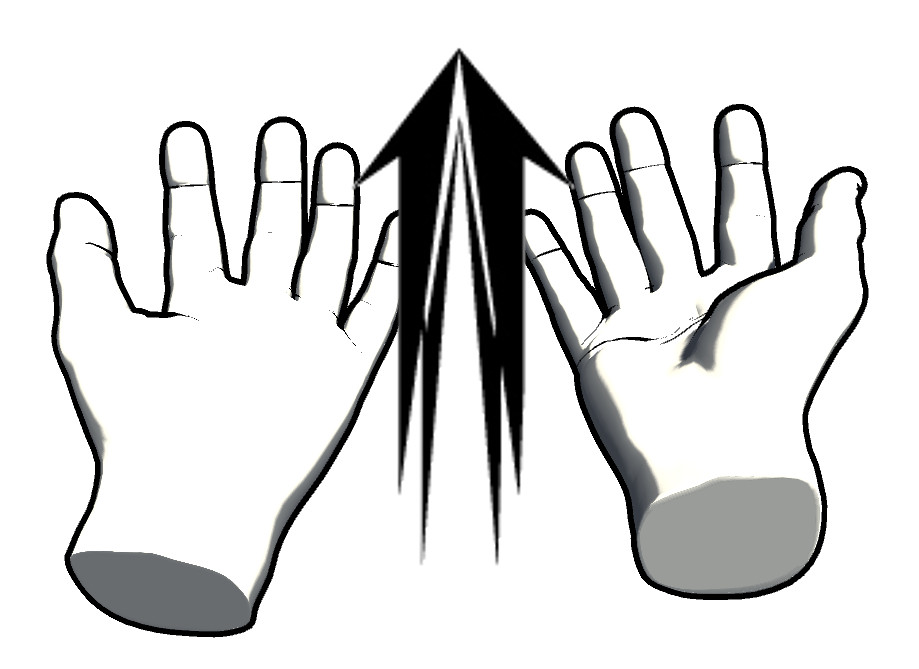
\includegraphics[height=0.08\textheight]{bilder/geste_menu} & Menu \\
		�bersicht & Scrollen & 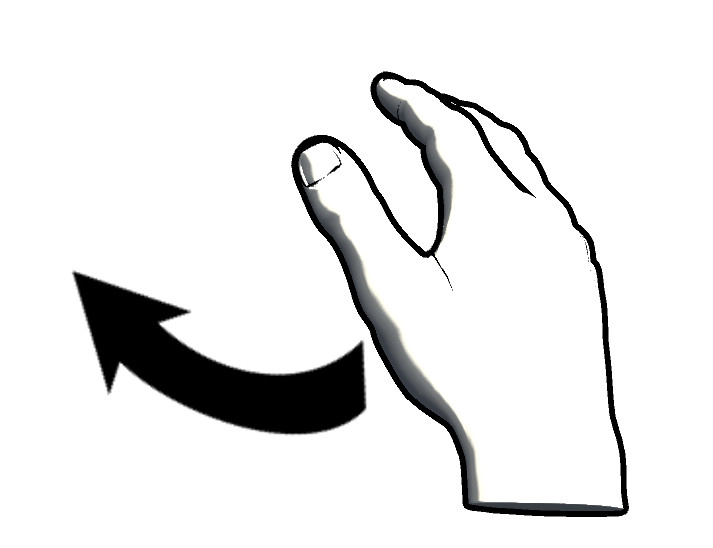
\includegraphics[height=0.08\textheight]{bilder/geste_scroll} & - \\
		Detail & Skalieren des aktiven Bildes & 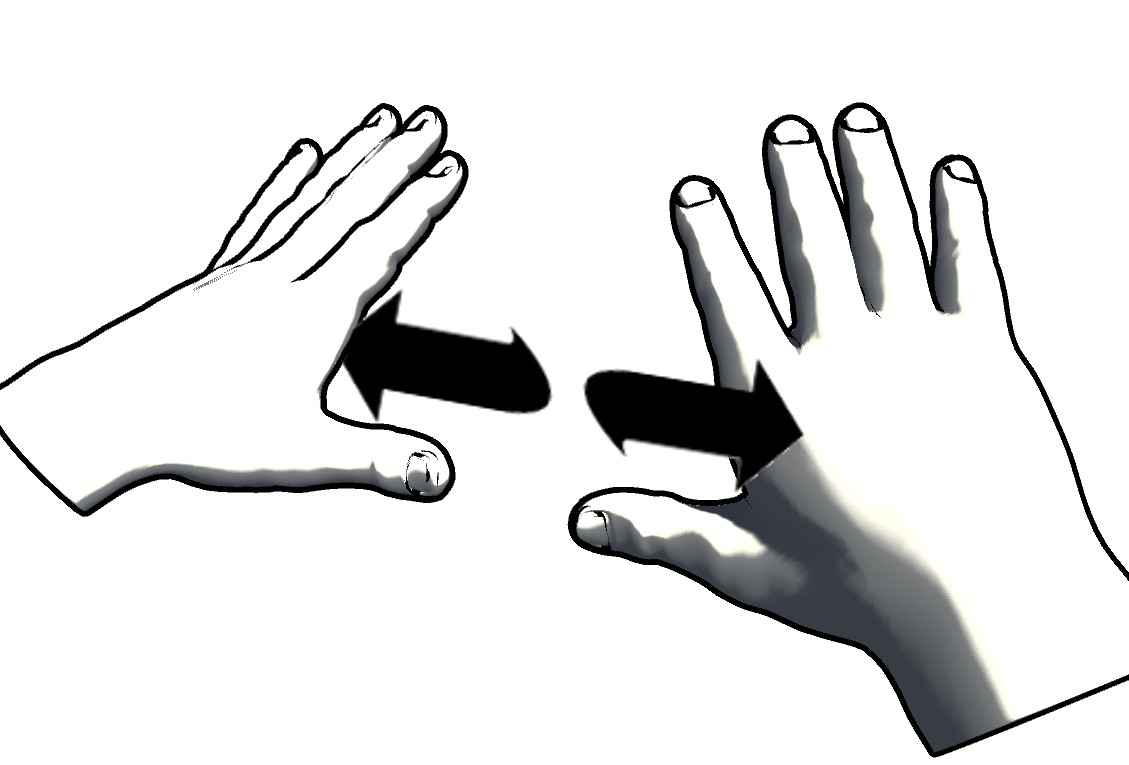
\includegraphics[height=0.08\textheight]{bilder/geste_scale} & - \\
		Detail & Rotieren des aktiven Bildes & 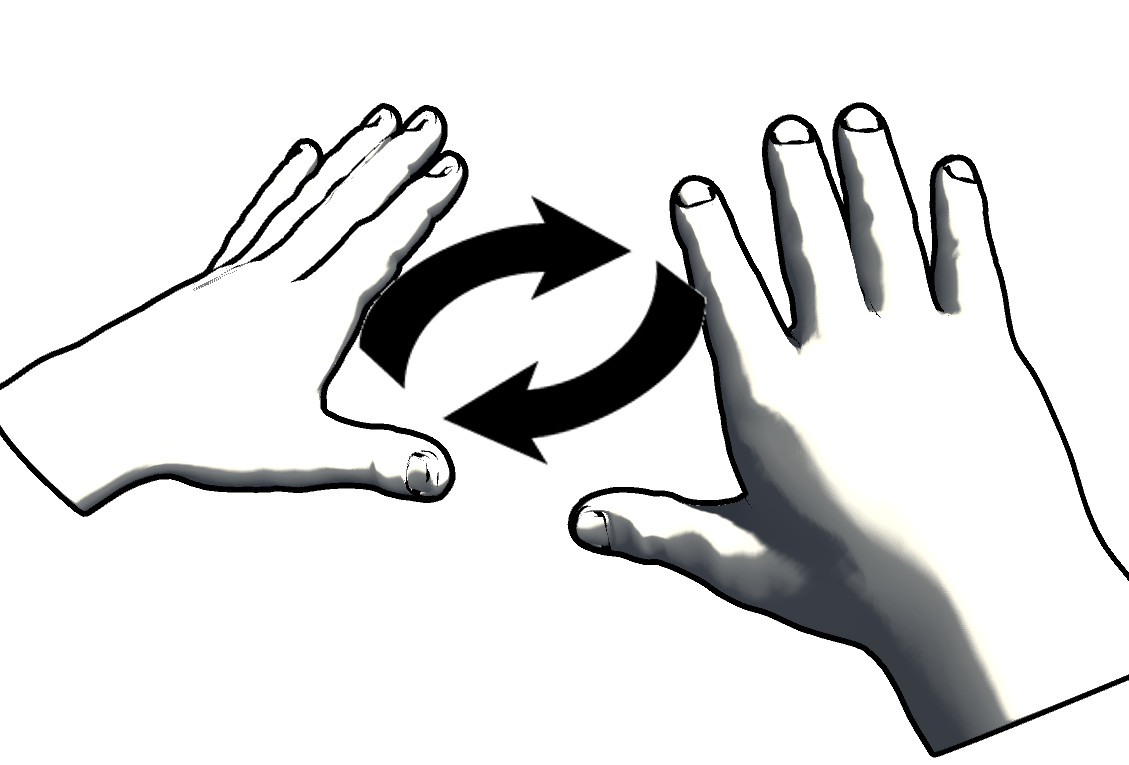
\includegraphics[height=0.08\textheight]{bilder/geste_rotate} & - \\
		�berall & Anzeigen von kontextsensitiven Statistiken & 
\includegraphics[height=0.08\textheight]{bilder/geste_statistics} & - \\
		Dialog & Annehmen / Ablehnen & 
\includegraphics[height=0.08\textheight]{bilder/geste_daumen} & - \\
		Detail & Ansicht verlassen & 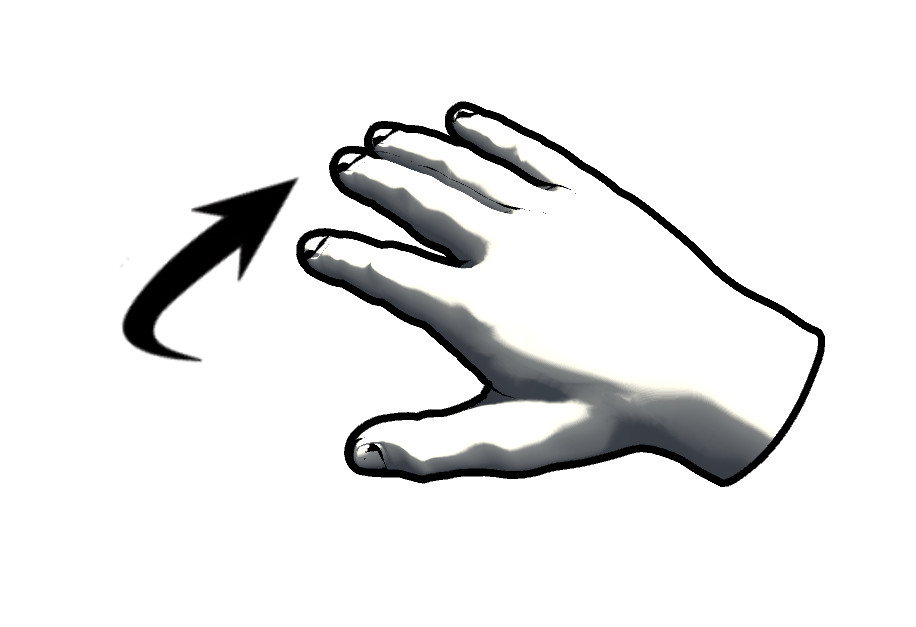
\includegraphics[height=0.08\textheight]{bilder/geste_weg} & - \\
	\end{tabular}
\end{table}

\chapter{Prototyp}

In der Vorbereitungsphase wurde ein Prototyp geschrieben, um zu testen, ob Unity in der Lage ist, Bilder und Musik so zu manipulieren, wie es die Anforderungen verlangen.

\section{Implementierung}

Der Prototyp besteht aus zwei Teilen: dem Unity-Programm und dem Indexer, der im 
Hintergrund Infos �ber Dateien sammelt. Zwischen den beiden Prozessen gibt es eine 
dateibasierte SQLite Datenbank, auf die mit normalem SQL oder ORM-Modellen zugegriffen 
werden kann.

Um Bilddateien zu analysieren, wird ImageMagick, welches bereits eine Vielzahl von 
Kennwerten zur�ckgibt, verwendet, da dieses �ber ein praktisches C\#-Interface 
verf�gt.

Musikdateien werden noch nicht analysiert. Dies kann jedoch mithilfe des jMIR-Projekts, der VAMP-Plugins und der Echo Nest API erreicht werden. Die Visualisierung der Musik wurde mit der NAudio Library realisiert - es ist allerdings m�glich, die n�tigen Werte direkt �ber die Unity-API zu ermitteln.

Alles in allem zeigt das Unity-Programm, dass es ohne Ruckeln m�glich ist, 100 Bilder zu laden und zu 
sortieren. Die anf�nglichen +100 Draw-Calls konnten auf 2 reduziert werden.

\section{Probleme}

In Sachen Bilder gibt es ein Problem, das es zu �berwinden gilt: Unity erlaubt es nicht, 
Texturen asynchron zu laden. Texturen der Gr�sse 256x256 brauchen nach einer Optimierung 
etwa 1ms zum Laden, was f�r eine Framerate von 60fps noch verkraftbar ist. Gr�ssere 
Texturen (512, 1024) erreichen jedoch schnell eine Ladezeit von 18-50ms, was sich 
langsam aber sicher bemerkbar macht.

Eine M�glichkeit dieses Problem zu l�sen, findet sich in den nativen Plugins: Es ist in Unity 
m�glich, DirectX (oder OpenGL) Code in C++ zu schreiben. Mit dieser Methode k�nnte man evtl. 
die Texturen besser allozieren.

Einfacher w�re es allerdings, alle n�tigen Bilder einfach vorzuladen.
\chapter{Organisation}

Dieses Kapitel beschreibt kurz die Stakeholder des Projekts sowie den allgemeinen Aufbau.

\section{Projektbeteiligte}

\begin{table}[H]
	\centering
	\begin{tabular}{p{0.2\textwidth} p{0.3\textwidth} p{0.3\textwidth}}
	\textbf{Name} & \textbf{Funktion} & \textbf{E-Mail Adresse} \\ \midrule
	Simon Meer & Student & simon.meer@students.bfh.ch \\
	Prof. Urs K�nzler & Betreuer & urs.kuenzler@bfh.ch \\
	Yves Petitpierre & Experte & ? \\
	\end{tabular}
\end{table}

\section{Projektmanagement}

Meetings zwischen dem Studenten und dem Betreuer finden jeden zweiten Mittwoch in Biel statt.

Das Projekt wird innerhalb eines Git-Projektes gef�hrt und im Laufe des Projekts entweder auf GitHub.com oder auf das interne Projektmanagement-Tool migriert.

Gearbeitet wird durch den Studenten Montags bis Donnerstags an einem Arbeitsplatz im CPVR Labor in Biel.

\section{Zeitplan}


\chapter{Testszenarien}

Dieses Kapitel definiert eine Reihe von Tests, mit denen das Projekt gepr�ft werden kann und soll.

\section{Indexer}

\begin{description}
	\item [T1 (Anforderung 6.1)] Der Benutzer f�gt seine ``Eigenen Bilder'' und seinen Windows-Ordner zur Library hinzu.
	\item [ $\blacktriangleright$] Der Indexer durchl�uft den Ordner fehlerfrei und die Anzahl indexierter Files, die er ausgibt, stimmt. 
	\item [T2 (Anforderung 6.2)] Der Benutzer �ffnet die Applikation.
	\item [ $\blacktriangleright$] Alle hinzugef�gten Bilder werden angezeigt und sind korrekt sortiert.
	\item [T3 (Anforderung 6.3)] Der Benutzer schliesst die Applikation und l�scht den Windows-Ordner von der Library und startet den Indexer.
	\item [ $\blacktriangleright$] Die Applikation zeigt beim n�chsten Start nur noch die Dateien im Ordner ``Eigene Bilder''.
\end{description}

\section{Bilder}

\begin{description}
	\item [$\bullet$] Der Benutzer f�gt seine ``Eigenen Bilder'' zur Library hinzu.
	\item [T1 (Anforderung 2.1)] Der Benutzer �ffnet die Applikation IMVR.
		\item [ $\blacktriangleright$] Ein 3D-Karussell (oder anders 3D-Konstrukt) mit seinen Bildern wird angezeigt.
	\item [T2 (Anforderung 2.2)] Der Benutzer �ffnet das Men� und sortiert nach Helligkeit.
		\item [ $\blacktriangleright$] Die Elemente werden neu sortiert und erscheinen geordnet nach Helligkeit.
	\item [T3 (Anforderung 2.4)] Der Benutzer ber�hrt mit den H�nden eines der Bilder.
		\item [ $\blacktriangleright$] Die �bersicht verblasst und das selektierte Bild wird vergr�ssert.
	\item [T4 (Anforderung 3.1)] Der Benutzer bewegt seine H�nde auseinander entsprechend der Gestentabelle.
		\item [ $\blacktriangleright$] Das Bild vergr�ssert sich entsprechend.
	\item [T5)] Der Benutzer wischt mit der Hand entsprechend der Gestentabelle.
		\item [ $\blacktriangleright$] Die Detailansicht wird verlassen und die �bersicht kommt wieder in den Vordergrund.
\end{description}

\section{Musik}

\begin{description}
	\item [T1 (Anforderung 4.1)] Der Benutzer f�gt seine ``Eigene Musik'' zur Library hinzu und startet den Indexer.
	\item [ $\blacktriangleright$] Alle MP3 Dateien mit korrekten ID3-Tags werden laut Log erkannt.
	\item [T2 (Anforderung 4.2)] Der Benutzer �ffnet die Applikation und wechselt in den Musikmodus.
	\item [ $\blacktriangleright$] Die soeben hinzugef�gte Musik erscheint alphabetisch geordnet.
	\item [T4 (Anforderung 1.5)] Der Benutzer �ffnet das Hauptmen� und beendet die Applikation.
		\item [ $\blacktriangleright$] Die Applikation fragt einmal nach und beendet dann.
\end{description}


%---------------------------------------------------------------------------

% Selbst�ndigkeitserkl�rung
%---------------------------------------------------------------------------
%\cleardoublepage
%\phantomsection 
%\addcontentsline{toc}{chapter}{Selbst�ndigkeitserkl�rung}
%\chapter*{Selbst�ndigkeitserkl�rung}
\label{chap:selbstaendigkeitserklaerung}

\vspace*{10mm} 

Ich/wir best�tige/n, dass ich/wir die vorliegende Arbeit selbstst�ndig und ohne Benutzung anderer als der im Literaturverzeichnis angegebenen Quellen und Hilfsmittel angefertigt habe/n. S�mtliche Textstellen, die nicht von mir/uns stammen, sind als Zitate gekennzeichnet und mit dem genauen Hinweis auf ihre Herkunft versehen. 

\vspace{15mm}

\begin{tabbing}
xxxxxxxxxxxxxxxxxxxxxxxxx\=xxxxxxxxxxxxxxxxxxxxxxxxxxxxxx\=xxxxxxxxxxxxxxxxxxxxxxxxxxxxxx\kill
Ort, Datum:		\> [Biel/Burgdorf], \versiondate \\ \\ 
Namen Vornamen:	\> [Test Peter] 	\> [M�ster R�s�] \\ \\ \\ \\ 
Unterschriften:	\> ......................................\> ...................................... \\
\end{tabbing}

%---------------------------------------------------------------------------

% Glossary
%---------------------------------------------------------------------------
\cleardoublepage
\phantomsection 
\addcontentsline{toc}{chapter}{Glossar}
\renewcommand{\glossaryname}{Glossar}
\printglossary

%---------------------------------------------------------------------------

% Bibliography
%---------------------------------------------------------------------------
%\cleardoublepage
%\phantomsection 
%\addcontentsline{toc}{chapter}{Literaturverzeichnis}
%\bibliographystyle{IEEEtranS}
%\bibliography{datenbanken/bibliography}{}
%---------------------------------------------------------------------------

% Listings
%---------------------------------------------------------------------------
%\cleardoublepage
%\phantomsection 
%\addcontentsline{toc}{chapter}{Abbildungsverzeichnis}
%\listoffigures
%\cleardoublepage
%\phantomsection 
%\addcontentsline{toc}{chapter}{Tabellenverzeichnis}
%\listoftables
%---------------------------------------------------------------------------

% Index
%---------------------------------------------------------------------------
\cleardoublepage
\phantomsection 
\addcontentsline{toc}{chapter}{Stichwortverzeichnis}
\renewcommand{\indexname}{Stichwortverzeichnis}
\printindex
%---------------------------------------------------------------------------

% Attachment:
%---------------------------------------------------------------------------
%\appendix
%\settocdepth{section}
%\chapter{Beliebiger Anhang}
\label{chap:bel_anhang}

Phasellus eget velit massa, sed faucibus nisi. Etiam tincidunt libero viverra lorem bibendum ut rutrum nisi volutpat. Donec non quam vitae lacus egestas suscipit at eu nisi. Maecenas non orci risus, at egestas tellus. Vivamus quis est pretium mauris fermentum consectetur. Cras non dolor vitae nulla molestie facilisis. Aliquam euismod nisl eget risus pretium non suscipit nulla feugiat. Nam in tortor sapien. Nam lectus nibh, laoreet eu ultrices nec, consequat nec sem. Nulla leo turpis, suscipit in vulputate a, dapibus molestie quam. Vestibulum pretium, purus sed suscipit tempus, turpis purus fermentum diam, id cursus enim mi a tortor. Proin imperdiet varius pellentesque. Nam congue, enim sit amet iaculis venenatis, dui neque ornare purus, laoreet porttitor nunc justo vel velit. Suspendisse potenti. Nulla facilisi.

%\chapter{Weiterer Anhang}
\label{chap:anhang_B}

\section{Test 1}
Phasellus eget velit massa, sed faucibus nisi. Etiam tincidunt libero viverra lorem bibendum ut rutrum nisi volutpat. Donec non quam vitae lacus egestas suscipit at eu nisi. Maecenas non orci risus, at egestas tellus. Vivamus quis est pretium mauris fermentum consectetur. Cras non dolor vitae nulla molestie facilisis. Aliquam euismod nisl eget risus pretium non suscipit nulla feugiat. Nam in tortor sapien. 

\subsection{Umfeld}
Nam lectus nibh, laoreet eu ultrices nec, consequat nec sem. Nulla leo turpis, suscipit in vulputate a, dapibus molestie quam. Vestibulum pretium, purus sed suscipit tempus, turpis purus fermentum diam, id cursus enim mi a tortor. Proin imperdiet varius pellentesque. Nam congue, enim sit amet iaculis venenatis, dui neque ornare purus, laoreet porttitor nunc justo vel velit. Suspendisse potenti. Nulla facilisi.

%\chapter{Inhalt der CD-ROM}
\label{chap:Inhalt_CDROM}

Inhaltsverzeichnis der beiliegenden CD-ROM, ev. Verzeichnisbaum, etc.
%---------------------------------------------------------------------------

%---------------------------------------------------------------------------
\end{document}

